\documentclass{article}

\usepackage{epigraph}
\usepackage{tikz}

\tikzstyle{box} = [rectangle, minimum width=3cm, minimum height=1cm, draw=black]
\tikzstyle{arrow} = [thick,->,>=stealth]

\title{On Chess Improvement}
\date{10 December 2023}

\begin{document}
\maketitle
\epigraph{I know I know nothing.}{Socrates}
\tableofcontents


\section{Introduction}
If in 20 days I had to become New Zealand Chess Champion, what would be the optimal strategy?

We are unaware on what we need to know, and thus we do not act upon it. This article aims to identify what we do not know, and how to train on what we know we do not know.

\section{The Components of Chess}
As with all large projects, it is essential to break it down into smaller parts. This allows for "rotating focus" (Benjamin Keep), where complex skills are most effectively learnt by focusing on one component at once. There are many ways to break down chess, however the diagram below shows one that is simple, complete, and useful. \\

\begin{center}
  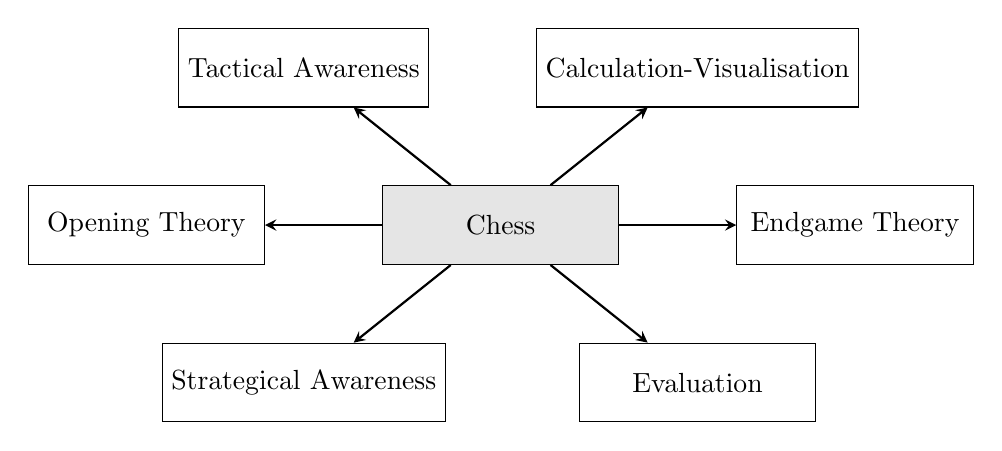
\begin{tikzpicture}
    \node (1) [box] at (0,0) {Tactical Awareness};
    \node (2) [box] at (5,0) {Calculation-Visualisation};
    \node (3) [box] at (-2,-2) {Opening Theory};
    \node (4) [box] at (7, -2) {Endgame Theory};
    \node (5) [box] at (0,-4) {Strategical Awareness};
    \node (6) [box] at (5,-4) {Evaluation};
    \node (Chess) [box, fill=gray!20] at (2.5, -2) {Chess};

    \draw[arrow] (Chess) -- (1);
    \draw[arrow] (Chess) -- (2);
    \draw[arrow] (Chess) -- (3);
    \draw[arrow] (Chess) -- (4);
    \draw[arrow] (Chess) -- (5);
    \draw[arrow] (Chess) -- (6);
  \end{tikzpicture}
\end{center}

A section will be devoted to the study of each. Very importantly, there be a strong focus on how to train a combination of components, often omitted from mainstream methods.


\section{Ineffective Methods}
Mainstream methods usually have multiple of the following flaws. Below are issues that may occur either during training or how it may impact their performance.
\subsection{On Tactics}
\begin{itemize}
  \item The learner does not know certain themes, and will not find them in their game.
  \item The learner incompetently understands how tactics may arise in the future, as they have been solely trained in positions with successful tactics.
  \item The learner views tactics as a pattern which randomly appears in the position. They are unable to use tactics to faciliate ambitious strategies.
  \item The learner submits ``leap of faith" answers, without fully calculating whether the tactic will be successful. A small change in the position disallowing the tactic will go unnoticed to the learner.
\end{itemize}
\subsection{On Calculation and Visualisation}
\begin{itemize}
  \item The learner does not know that their method of calculation and visualisation is inefficient. This may be their order of calculation, their organisation of lines, or how their imagine pieces moving on the board.
  \item The learner does not calculate with full accuracy. They can calculate a line and misplace a piece, however it is not tested by the method.
  \item The learner can work through a line, however it is so slow and arduous that they are unable to intertwined it with their general positional awareness.
\end{itemize}
\subsection{On Openings}
\begin{itemize}
  \item The learner does not know what lines are critical. Critical lines are where the position requires large calculations to decide a move, so prior knowledge can save great time.
  \item The learner does not remember enough critical lines. This may be because the method may force them to remember too many non-critical lines.
  \item The learner does not understand the nature of the position, how small changes may affect the position.
\end{itemize}
\subsection{On Endgame Theory}
\begin{itemize}
  \item The learner does not know the endgames they will go wrong in.
  \item The learner fails to remember a theoretical endgame. They also may inefficiently study uncommon endgames.
\end{itemize}
\subsection{On Strategical Awareness}
\begin{itemize}
  \item The learner does not know what strategies they do not know.
  \item The learner does not know when to apply a strategy they do know.
\end{itemize}

Evaluation is rarely trained, so there is no subsection on it. By reading these flaws, we may identify that the method may not train us on what we do not know, or train us ineffectively. We can now begin to discuss the optimal training methods.

\section{Tactical Awareness}
Training is only useful if it has changed what we have played compared to before the training.

We can begin on this axiom, and work our ways backwards towards the most effective training method.

\begin{center}
  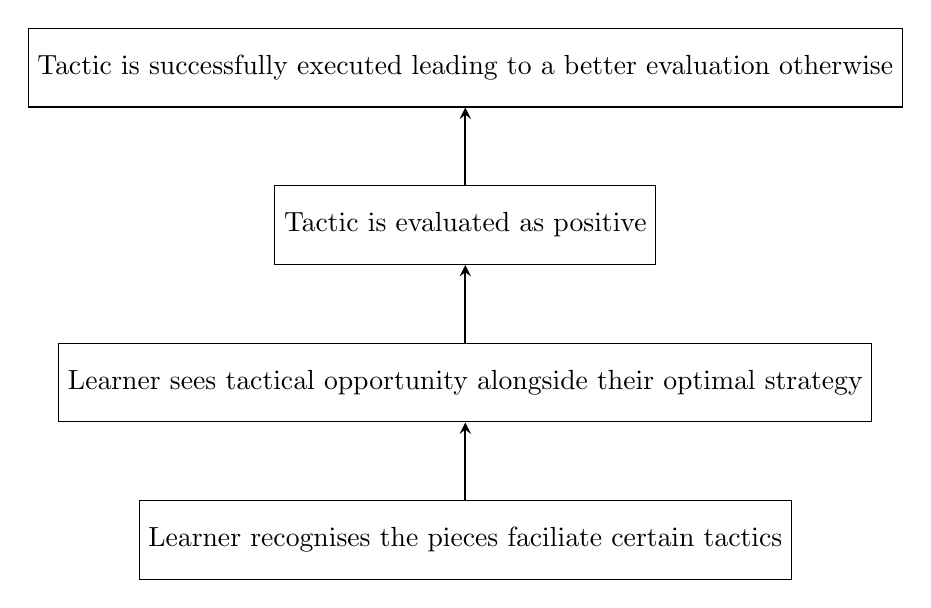
\begin{tikzpicture}[node distance=2cm]
    \node (1) [box] {Tactic is successfully executed leading to a better evaluation otherwise};
    \node (2) [box, below of=1] {Tactic is evaluated as positive};
    \node (3) [box, below of=2] {Learner sees tactical opportunity alongside their optimal strategy};
    \node (4) [box, below of=3] {Learner recognises the pieces faciliate certain tactics};

    \draw[arrow] (2) -- (1);
    \draw[arrow] (3) -- (2);
    \draw[arrow] (4) -- (3);
  \end{tikzpicture}
\end{center}

In order to play a successful tactic, it must be calculated and evaluated the tactic as positive, which improvement will be discussed in other sections. Before then, the tactic must be seen - this is the core of tactical awareness. To see a tactic, the learner must recognise how pieces influence the tactics possible.

Luckily, total simulation of this is possible. The learner can open any position they want to improve tactics in, and begin to search for all tactics that they can find that may arise in a few moves. This defines that boundary of what they know. Then a program can tell the learner of all possible tactics in the position, to explore what they do not know.

Overtime, the learner can record the \% of tactics they have found. This can quantify the skill of the learner and show a sign of improvement. In order to ensure there the learner identifies what they do not know, they must test against a wide variety of positions. Also limitations of the program must be identified to ensure special types of tactics are learnt separately.



\end{document}